\section{Event Storming}\label{sec:event-storming}
In diesem Unterkapitel werden die grundlegenden Prinzipien und Ziele des \ac{DDD} erläutert, welche von Vaughn Vernon in seinem Buch
\textit{Domain-Driven Design Distilled} definiert hat.\cite*{dddd}
Nachdem diese Grundlage vorhanden ist, wird darauf aufbauend erklärt, welche Symbiose aus dem \ac{DDD} und dem \ac{ES} entsteht und wie
dies zu einer Softwareentwicklung beiträgt.
Zur Veranschaulichung eines Event Stormings wird ein von Alberto Brandolini beschriebener \ac{ES}-Workshop genutzt.
Abschließend werden die Änderungen und Erweiterungen, welche im Kontext dieser Arbeit vorgenommen wurden, erklärt.

\subsection{Domain-Driven Design}\label{subsec:domain-driven-design}
Das \ac*{DDD} ist nicht nur für die erste Phase der Softwareentwicklung praktisch, sondern ebenso für das Umstrukturieren bestehender Projekte.
Ein grundlegendes Ziel des \ac{DDD} ist es ein Projekt in sogenannte \textit{Bounded Contexts} zu unterteilen und damit zu umgehen, dass
die Anwendung aus einem riesigen aufgeblähten Modell besteht.
Um dieses Ziel zu erreichen, ist es wichtig in Gesprächen mit Domänenexperten die wichtigsten Punkte eines \textit{Bounded Context} zu evaluieren.
Domänenexperten können in jedem Bereich eines Unternehmens gefunden werden.
Es ist nötig ein möglichst breites Spektrum an Personen zu haben, um den gesamten zu entwickelnden Prozess zu verstehen und für die Entwickler verständlich zu machen.
Dabei ist es wichtig, dass alle Personen, welche am Prozess des \ac{DDD} teilnehmen eine einheitliche Sprache zu entwickeln.
Diese einheitliche Sprache beschreibt Vernon als~\textit{Ubiquitous Language}.\footnote{Seite 7 in~\cite*{dddd}}
Eine allgegenwärtige Sprache (\textit{Ubiquitous Language}) zu entwickeln, ist ein fortlaufender Prozess.
Initial ist es wichtig, dass zwischen den verschiedenen Domänenexperten und den Entwicklern diese einheitliche Sprache entsteht, welche
nicht nur das Verständnis zwischen den beiden Parteien, sondern auch mit in das Modell einfließen soll.

\subsection{Event Storming}\label{subsec:allgemein}
Vernon selbst nennt Event Storming, als eine Möglichkeit um eine~\textit{Ubiquitous Language} zu entwickeln.\footnote{Seite 112, folgende in~\cite*{dddd}}
Event Storming wurde von Alberto Brandolini entwickelt und resultiert aus mangelnder Zeit während der Nutzung von \textit{event-driven modeling}.
\textit{Event-driven modeling} basiert ebenfalls auf Konversationen und konkreten Szenarien, allerdings mit der Verwendung von UML-Diagrammen zur Datenmodellierung.
Dies hatte zur Konsequenz, dass in Gesprächen ab einem bestimmten Punkt nur noch die Entwickler daran teilnahmen.
Brandolini verwarf UML-Diagramme und verwendete Haftnotizen und legte damit für das~\ac{ES}.\footnote{Seite 113 in~\cite*{dddd}}

In seinem Buch, \textit{Introducing EventStorming}, beschreibt Brandolini mehrere Event Storming Workshops und wie diese durchgeführt wurden.\cite*{introES}
Hierbei stellt sich heraus, dass Event Storming kein starres Konstrukt aus Abläufen ist, sondern je nach Kontext angepasst werden kann.
Dennoch gibt es Ähnlichkeiten, welche eine solide Grundlage für ein Event Storming Workshop bieten.\footnote{Seite 23 in~\cite*{introES}}
Neben einem grenzenlosen Platz zum Modellieren benötigt es genügend Marker und Haftnotizen in verschiedenen Formen und Farben.
Die teilnehmenden Domänenexperten benötigen eine kollaborative Einstellung zur Modellierung, ein offenes Miteinander ungeachtet ihrer Stellung.
Keine Grenzen zu dem Thema oder der Anwendung welche modelliert werden soll, um weitere Probleme oder Fragen zu lösen und beantworten zu können.
Ein Event Storming beginnt immer mit dem Erstellen von Domain Events und dem Platzieren dieser anhand eines Zeitstrahles.
Zudem müssen alle Beteiligten am fortlaufenden Verfeinern eines Modells interessiert sein, da ein \ac{ES}-Workshop zum Lernen und Verbessern
von Anwendungen gedacht ist.
Ein Event Storming Board nach einem solchen Workshop ist in Abbildung~\ref{fig:rlBoard} dargestellt.

\begin{figure}[h]
    \centering
    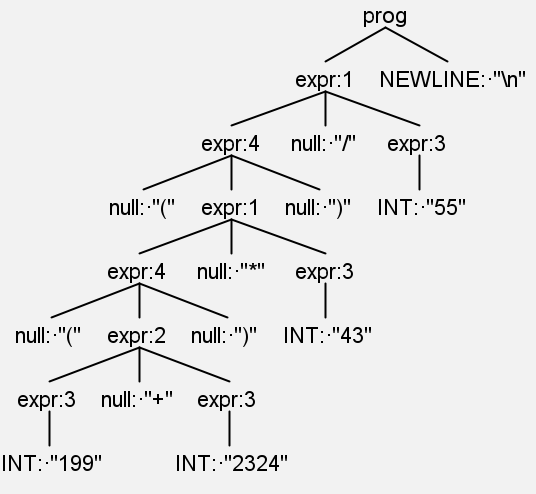
\includegraphics[width=0.5\textwidth]{images/2.2/parseTreeExample}
    \caption{Interner ParseTree}
    \label{fig:rlBoard}
\end{figure}

\todo{Fig beschreiben}

\todo{Verschiednene Arten der Benutzung -> Big picture, design level, ....}

\todo{Erweiterbarkeit von notes bezogen uf den kontext -> Überleitung zum nächsten kapitel}

\subsection{Erweiterung}\label{subsec:erweiterung}
\todo{Hier das vorherige Kapitel abwarten um alle Änderungen/Erweiterungen besser daran fest zu machen.}
\begin{itemize}
    \item Erweiterungen für Wirtschaft (Pages -> daraus generierte Mockups, abgehen von dem "Wir wollen keinen PC benutzen" des ES)
    \item Ideen für die Lehre (Wird in dieser Arbeit nicht näher beleuchtet, da es für den Beleg der Funktionalität nicht mehr möglich ist dies ausreichend in der Bearbeitungszeit zu machen)
    \item ES -> Ablauf von Schritten -> Albert -> Workflow (Arbeitsablauf) beschreibungen -> Mögliche Idee zum besseren Nahebringen von komplexeren Abläufen in Vorlesungen. (Verbildlichung)
\end{itemize}
